% !TeX document-id = {5530719d-34df-4dd8-b4b5-e6ed092c2b36}
% !TeX program = pdflatex
% !BIB program = biber
\documentclass[
sigconf,natbib=false
%,anonymous=true
]{acmart}

%\usepackage[subtle,bibnotes,charwidths,mathdisplays,indent,lists]{savetrees}

%\usepackage{fnpos}
%\usepackage{dblfnote}
%\usepackage{ftnright}

\usepackage[%
%false
]{anonymous-acm}

\usepackage{amsmath}
\let\openbox\relax
\usepackage{amsthm}
\newcommand\bmmax{2}
\usepackage{bm}

\usepackage[ruled,vlined]{algorithm2e}

% Get Booktab style ruling in algorithm blocks.
% Values shamelessly taken from egreg's answer in 
% https://tex.stackexchange.com/a/345745/82917
\makeatletter
\renewcommand*{\@algocf@pre@ruled}{\hrule height\heavyrulewidth depth0pt \kern\belowrulesep}
\renewcommand*{\algocf@caption@ruled}{\box\algocf@capbox\kern\aboverulesep\hrule height\lightrulewidth\kern\belowrulesep}
\renewcommand*{\@algocf@post@ruled}{\kern\aboverulesep\hrule height\heavyrulewidth\relax}
\makeatother

% Imports Ahoy

%\usepackage[dvipsnames]{xcolor}
%\usepackage{graphicx}
\usepackage{tikz}
\usepackage{varwidth}
\usetikzlibrary{arrows.meta, calc, fit, positioning}

\usepackage[title]{appendix}

\usepackage{etoolbox}
\usepackage[per-mode=symbol]{siunitx}
\robustify\bfseries
\robustify\emph
%\robustify\uline
\sisetup{detect-all, range-phrase=--, range-units=single, detect-weight=true, table-format=1.3}
\DeclareSIUnit{\packet}{p}

\makeatletter
\let\MYcaption\@makecaption
\makeatother

\usepackage[font=footnotesize]{subcaption}
\usepackage{awesomebox}

\makeatletter
\let\@makecaption\MYcaption
\makeatother

%\usepackage[basic]{complexity}
\usepackage[super,negative]{nth}

\usepackage[british]{babel}
\usepackage{csquotes}
\usepackage{pifont}

\usepackage{booktabs}
%\usepackage[
%activate={true,nocompatibility},
%final,
%tracking=true,
%kerning=true,spacing=true
%]{microtype}
%\microtypecontext{spacing=nonfrench}

\usepackage[maxnames=1,maxbibnames=1,mincrossrefs=99,sortcites,style=numeric-comp
%,backend=biber
]{biblatex}
\addbibresource{papers-off.bib}
\addbibresource{confs-off.bib}
\addbibresource{books-off.bib}
\addbibresource{rfc.bib}
\addbibresource{misc.bib}

\DeclareFieldFormat[inproceedings]{doi}{}
\DeclareFieldFormat[article]{doi}{}
\DeclareFieldFormat*{url}{}
%\DeclareFieldFormat[online]{url}{\mkbibacro{URL}\addcolon\space\url{#1}}
%\DeclareFieldFormat[report]{url}{\mkbibacro{URL}\addcolon\space\url{#1}}

%picky abt et al.
\usepackage{xpatch}

\usepackage{url}
\usepackage{hyperref}
\usepackage[nameinlink]{cleveref}
\newcommand{\crefrangeconjunction}{--}
\crefname{table}{table}{tables}

\DefineBibliographyStrings{english}{%
	andothers = {\emph{et al}\adddot}
}
\DeclareFieldFormat[inproceedings]{url}{}
\DeclareFieldFormat[article]{url}{}
%\DeclareFieldFormat[inproceedings]{doi}{}
%\DeclareFieldFormat[article]{doi}{}
\DeclareFieldFormat[inproceedings]{editor}{}
\DeclareFieldFormat[proceedings]{editor}{}
\DeclareFieldFormat[article]{editor}{}
\DeclareFieldFormat[inproceedings]{isbn}{}
\DeclareFieldFormat[proceedings]{isbn}{}
\DeclareFieldFormat[article]{isbn}{}

\newcommand{\fakepara}[1]{\noindent\textbf{#1:}}

% Official colours!

\definecolor{uofguniversityblue}{rgb}{0, 0.219608, 0.396078}

\definecolor{uofgheather}{rgb}{0.356863, 0.32549, 0.490196}
\definecolor{uofgaquamarine}{rgb}{0.603922, 0.72549, 0.678431}
\definecolor{uofgslate}{rgb}{0.309804, 0.34902, 0.380392}
\definecolor{uofgrose}{rgb}{0.823529, 0.470588, 0.709804}
\definecolor{uofgmocha}{rgb}{0.709804, 0.564706, 0.47451}

\definecolor{uofglawn}{rgb}{0.517647, 0.741176, 0}
\definecolor{uofgcobalt}{rgb}{0, 0.615686, 0.92549}
\definecolor{uofgturquoise}{rgb}{0, 0.709804, 0.819608}
\definecolor{uofgsunshine}{rgb}{1.0, 0.862745, 0.211765}
\definecolor{uofgpumpkin}{rgb}{1.0, 0.72549, 0.282353}
\definecolor{uofgthistle}{rgb}{0.584314, 0.070588, 0.447059}
\definecolor{uofgpillarbox}{rgb}{0.701961, 0.047059, 0}
\definecolor{uofglavendar}{rgb}{0.356863, 0.301961, 0.580392}

\definecolor{uofgsandstone}{rgb}{0.321569, 0.278431, 0.231373}
\definecolor{uofgforest}{rgb}{0, 0.317647, 0.2}
\definecolor{uofgburgundy}{rgb}{0.490196, 0.133333, 0.223529}
\definecolor{uofgrust}{rgb}{0.603922, 0.227451, 0.023529}

% End Imports

%\usepackage[english]{babel}
\usepackage{blindtext}

% Copyright
%\renewcommand\footnotetextcopyrightpermission[1]{} % removes footnote with conference info
%\setcopyright{none}
%\setcopyright{acmcopyright}
%\setcopyright{acmlicensed}
%\setcopyright{rightsretained}
%\setcopyright{usgov}
%\setcopyright{usgovmixed}
%\setcopyright{cagov}
%\setcopyright{cagovmixed}

%\settopmatter{printacmref=false, printccs=false, printfolios=true}
%\settopmatter{printfolios=true, printccs=true}
%\settopmatter{printacmref=false, printccs=true, printfolios=true}

\acmYear{2021}\copyrightyear{2021}
\acmConference[CoNEXT '21]{The 17th International Conference on emerging Networking EXperiments and Technologies}{December 7--10, 2021}{Virtual Event, Germany}
\acmBooktitle{The 17th International Conference on emerging Networking EXperiments and Technologies (CoNEXT '21), December 7--10, 2021, Virtual Event, Germany}
\acmPrice{15.00}
\acmDOI{10.1145/3485983.3493345}
\acmISBN{978-1-4503-9098-9/21/12}


\newcommand{\approach}{On Path Learning}
\newcommand{\approachshort}{OPaL}
\newcommand{\Coopfw}{\emph{CoOp}}
\newcommand{\coopfw}{\Coopfw}
\newcommand{\Indfw}{\emph{Ind}}
\newcommand{\indfw}{\Indfw}
\newcommand{\inring}{\textsc{In}}
\newcommand{\outring}{\textsc{Out}}

\makeatletter\let\expandableinput\@@input\makeatother
\newcommand{\cmark}{\ding{51}}%
\newcommand{\xmark}{\ding{55}}%

% make math easy
\newcommand{\acval}[3]{\ensuremath{\operatorname{\hat{q}}(#1, #2, #3)}}
\newcommand{\acvalblank}{\ensuremath{\operatorname{\hat{q}}(\cdot)}}
\newcommand{\wvec}[1]{\ensuremath{\bm{w}_{#1}}}

\newcounter{insightc}
\newenvironment{insight}
	{
		\begin{tipblock}\refstepcounter{insightc}\textbf{Insight \theinsightc:}\em
	}
	{
		\end{tipblock}
	}

\begin{document}
	\title{Poster: Online RL in the Programmable Dataplane with \approachshort{}}
	
%	\titlenote{Produces the permission block, and copyright information}
	%\subtitle{Extended Abstract}
	
%	\author{Paper \# XXX, XXX pages}
	 \author{Kyle A. Simpson}
	 \orcid{0000-0001-8068-9909}
	 \affiliation{%
	   \institution{University of Glasgow}
	   \city{Glasgow} 
	   \country{Scotland}
	 }
	 \email{k.simpson.1@research.gla.ac.uk}
	 \author{Dimitrios P. Pezaros}
\orcid{0000-0003-0939-378X}
	 \affiliation{%
	\institution{University of Glasgow}
	\city{Glasgow} 
	\country{Scotland}
}
\email{Dimitrios.Pezaros@gla.ac.uk}

\setlength{\abovecaptionskip}{5pt}
\setlength{\belowcaptionskip}{0pt}

\setlength{\textfloatsep}{3.0pt plus 0.0pt minus 3.0pt}
\setlength{\floatsep}{3.0pt plus 0.0pt minus 2.0pt}

\setlength{\dbltextfloatsep}{3.0pt plus 0.0pt minus 3.0pt}
\setlength{\dblfloatsep}{3.0pt plus 0.0pt minus 2.0pt}
	
% The default list of authors is too long for headers}
%\renewcommand{\shortauthors}{Simpson \emph{et al}.}
	
\begin{abstract}
%Automatic, data-driven networking is becoming more capable and widely researched, partly driven by the efficacy of \emph{Deep Reinforcement Learning} (DRL) algorithms.
%Yet the complexity of both DRL inference and learning force these tasks to be offloaded \emph{away from the dataplane} to hosts, harming latency-sensitive applications.
%Online learning of such policies cannot occur in the dataplane, despite being useful techniques when problems evolve or are hard to model.

Reinforcement learning (RL) is a key tool in data-driven networking for learning to control systems online.
While recent research has shown how to offload machine learning tasks to the dataplane (reducing processing latency), online learning remains an open challenge unless the model is moved back to a host CPU, harming latency-sensitive applications.
Our poster introduces \emph{\approachshort{}}---\approach{}---the first work to bring \emph{online reinforcement learning} to the dataplane.
\approachshort{} makes online learning possible in SmartNIC/NPU hardware by returning to classical RL techniques---avoiding neural networks.
This simplifies update logic, enabling online learning, and benefits well from the parallelism common to SmartNICs.
We show that our implementation on Netronome SmartNIC hardware offers concrete latency improvements over host execution.

%Compared to offloading, we achieve a \SI{21}{$\times$} reduction in \num{99.99}\nthscript{th} tail inference times to \SI{34}{\micro\second}, and \SI{9.9}{$\times$} improvement in online throughput for real-world policy designs.
%In-NIC execution eliminates PCIe transfers, and our asynchronous compute model ensures minimal impact on traffic carried by a co-hosted P4 dataplane.
%\approachshort{}'s design scales with additional resources at compile-time to improve upon both decision latency and throughput, improving on offloading, and are quickly reconfigurable at runtime compared to reinstalling device firmware.

\end{abstract}

\begin{CCSXML}
	<ccs2012>
	<concept>
	<concept_id>10003033.10003068.10003069</concept_id>
	<concept_desc>Networks~Data path algorithms</concept_desc>
	<concept_significance>500</concept_significance>
	</concept>
	<concept>
	<concept_id>10003033.10003099.10003102</concept_id>
	<concept_desc>Networks~Programmable networks</concept_desc>
	<concept_significance>500</concept_significance>
	</concept>
	<concept>
	<concept_id>10003752.10010070.10010071.10010261</concept_id>
	<concept_desc>Theory of computation~Reinforcement learning</concept_desc>
	<concept_significance>300</concept_significance>
	</concept>
	<concept>
	<concept_id>10010147.10010257.10010258.10010261</concept_id>
	<concept_desc>Computing methodologies~Reinforcement learning</concept_desc>
	<concept_significance>500</concept_significance>
	</concept>
	</ccs2012>
\end{CCSXML}

\ccsdesc[500]{Networks~Data path algorithms}
\ccsdesc[500]{Networks~Programmable networks}
\ccsdesc[500]{Computing methodologies~Reinforcement learning}

%\keywords{ACM proceedings, \LaTeX, text tagging}
	
\maketitle

\setlength{\aweboxleftmargin}{0.12\linewidth}
\setlength{\aweboxcontentwidth}{1.97\linewidth}

%\vspace{-1em}
\section{Introduction}
\begin{figure}
	\centering
		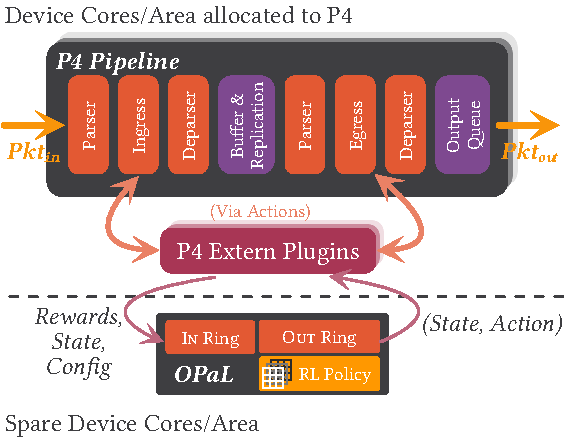
\includegraphics[keepaspectratio, width=0.8\linewidth]{figures/arch-with-p4}
		\caption{\approachshort{} brings low-latency, online reinforcement learning to SoC- and NPU-based SmartNICs. Classical RL policy methods are the key to making this computationally feasible.\label{fig:netro-arch}}
\end{figure}
\begin{figure}
	\centering
%	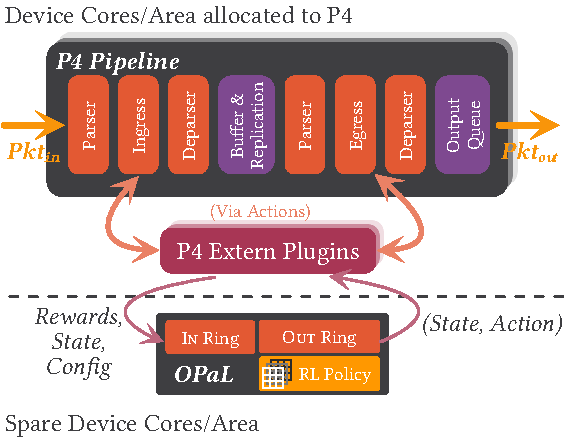
\includegraphics[keepaspectratio, width=0.6875\linewidth]{figures/arch-with-p4}
%	\caption{\approachshort{} brings low-latency, online reinforcement learning directly to the dataplane. SoC- and NetFPGA-based SmartNIC devices expose spare compute---making in-situ, asynchronous processing and learning possible alongside P4 dataplanes. Classical RL policy methods are the key to making this computationally feasible.\label{fig:netro-arch}}
	\centering
	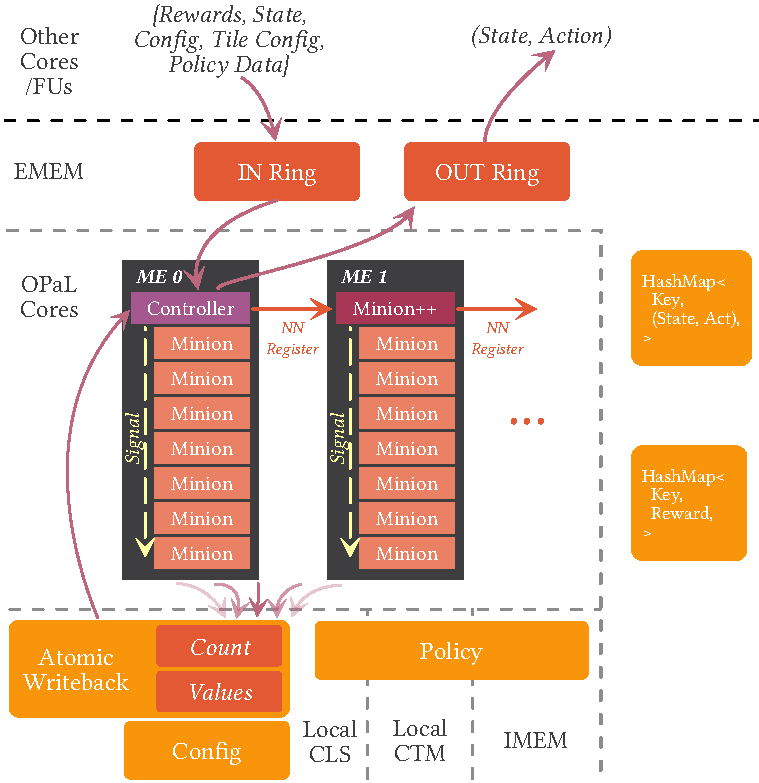
\includegraphics[keepaspectratio, width=0.8\linewidth]{figures/coop}
	\caption{Parallel policy execution. A single \emph{controller} delegates RL computation and updates to many \emph{minion} threads, using a shared atomic writeback.\label{fig:single-and-parallel:parallel}}
\end{figure}
Automatic network optimisation, control, and defence are becoming commonplace through data-driven techniques such as RL methods, where every change and its effects improve future decisions made by an agent.
In tandem, P4~\parencite{DBLP:journals/ccr/BosshartDGIMRSTVVW14} and \emph{programmable dataplane} hardware have inspired explosive growth and interest in the research community surrounding in-network computation and offloading.
This ecosystem exposes not only runtime reconfigurable packet processing, but per-packet and per-flow traffic measurement state that can greatly aid network operation~\parencite{DBLP:conf/sosr/GhasemiBR17}.

%Parallel to this, P4~\parencite{DBLP:journals/ccr/BosshartDGIMRSTVVW14} and programmable dataplane hardware~\parencite{DBLP:journals/micro/ZilbermanACM14, netronome-smartnic, xilinx-alveo, barefoot-intel} have inspired explosive growth and interest in the research community surrounding in-network computation and offloading.
%This has manifested in novel uses of programmable dataplane hardware to accelerate distributed tasks, fine-grained traffic measurement~\parencite{DBLP:conf/sigcomm/GuptaHCFRW18,DBLP:conf/sigcomm/ChenFKRR18,DBLP:conf/sosr/GhasemiBR17}, or per-packet processing.
%The latter is particularly attractive due to the costs of offloading to commodity host machines; input data must cross the PCIe bus several times, throughput requirements often impose the use of batching, and dedicated accelerators must again be contacted over PCIe~\parencite{DBLP:journals/corr/abs-2009-02353}.
%Additionally, in multi-tenant environments, IOMMU contention for both NICs and inference accelerators may impact tail latencies~\parencite{DBLP:conf/sigcomm/NeugebauerAZAL018}.
%In response, we have seen non-neural ML techniques~\parencite{DBLP:conf/hotnets/XiongZ19}, neural networks~\parencite{DBLP:conf/sigcomm/SanvitoSB18,DBLP:journals/corr/abs-1801-05731,DBLP:journals/corr/abs-2009-02353,langlet-ml-netronome}, and hardware design proposals for CGRA-based map-reduce blocks~\parencite{DBLP:journals/corr/abs-2002-08987} \emph{directly in the dataplane}.
%These works have shown the value in in-network ML: high-throughput, low latency response to network changes, particularly when co-hosted with state extraction.

%---

%?? Do we want concrete examples of things `pushed down the stack'?
%
%?? Consider a DDoS prevention system...
%?? in the face of new data, Able to start learning again in microseconds
\fakepara{Machine learning in the dataplane}
To process this fine-grained state both at line rate \emph{and} at low latency, there has been keen interest in executing ML models in the dataplane~\parencite{DBLP:conf/hotnets/XiongZ19,DBLP:journals/corr/abs-2009-02353}.
Works in this category, while powerful, operate by converting a \emph{pre-trained} model into a suitable representation, such as a binary neural network or string of match-action tables.
%These works have shown the value of in-network ML: high-throughput, low latency response to network changes.
These can react to on-device state, yet the missing piece of the puzzle is learning and updating these ML analyses \emph{online}, without deferring to another machine in the network.
%Training these models online and in-network is an exciting (and challenging) lacuna in the field that \emph{has yet to be addressed by the community}.
This lacuna has yet to be addressed by the community.

\fakepara{Problems of online training}
Programmable dataplane hardware, being designed solely for efficient packet processing, lacks floating-point arithmetic support, even in the case of more general purpose NPU-type SmartNICs.
Additionally, deep neural network training relies on backpropagation, can require memorizing many a sizeable replay buffer for RL, and needs many mini-batches of data for stable training.
The natural solution is to pass training data to a host machine or dedicated accelerator, yet this adds delays in crossing the PCIe bus, kernel-user handover, and buffering---adding latency while learning.
The above (NIC-suitable) inference schemes still must be trained offline, even though their data formats solve the issue of floating point use.
Online learning thus requires careful choices in sample data formats and the learned function approximation scheme.

\section{\approachshort{}'s design}
\approachshort{} makes RL workloads feasible on SmartNICs by using quantised fixed-point representations of action values, tile-coded policies, and one-step temporal-difference RL algorithms such as Sarsa~\parencite{RL2E}.
These allow us to evaluate and update policies using \emph{only integer arithmetic}, and are computationally simple.
We observe that tile coded inference is a map-reduce problem (\cref{fig:par-tilecode}), and thus over integers admits a novel \emph{wait-free Sarsa} RL algorithm (exploiting the parallelism built in to SmartNICs).
While these functions have lower theoretical model capacity, they do not require batches of inputs to learn in a stable way, negating the memory needed to store experience replays or minibatches.

\fakepara{Interacting with \approachshort{}}
To prevent packet stalls but maintain access to fine-grained state, \approachshort{} places RL execution on-NIC, \emph{but off the main packet path}, parallel to the main dataplane (\cref{fig:netro-arch}).
The P4 (or device-specific) dataplane pushes state vectors and reward measurements to \approachshort{}'s \inring{} ring, and pulls output actions when it is able to, imposing minimal impact on carried traffic for both bump-in-the-wire deployments and at end-points.
Once an action is enqueued on its \outring{} ring, \approachshort{} updates its policy.

\fakepara{Inference/Updates}
State is sent to a set of packet processing threads, which compute hit tiles from a locally held work set.
During inference, these threads atomically add values to a shared action preference list, while tile-coding guarantees that policy updates proceed without data races (\cref{fig:single-and-parallel:parallel}).
In the case of our Netronome implementation, these run on lightweight cores known as \emph{microengines} (MEs)---which could be substituted for suitable FUs on CGRA/FPGA hardware.
Additionally, we have a single-threaded implementation, \indfw, which forgoes this cooperative model to maximise offline throughput (by having many parallel single-threaded agents).

\begin{figure}
	\centering
	\resizebox{0.6\linewidth}{!}{
		\begin{tikzpicture}
			\node at (0,0) {
				\begin{tikzpicture}
					\draw[step=0.5cm,color=uofgcobalt,opacity=0.7,shift={(0,0)},label=above:{Tiling 0}] (-0.5,-0.5) grid (1,1);
					\fill[uofgcobalt,opacity=0.5] (0.5,-0.5) rectangle (1,0);
					\node[color=uofgcobalt] (t1g) at (0,1.2) {\footnotesize Tiling 1};
					
					\draw[step=0.5cm,color=uofgpumpkin,opacity=0.9,shift={(0.25,-0.25)},label=above:{Tiling 1}] (-0.5,-0.5) grid (1,1);
					\fill[uofgpumpkin,opacity=0.5,shift={(0.25,-0.25)}] (0,0) rectangle (0.5,0.5);
					\node[color=uofgpumpkin!50!uofgrust] (t2g) at (0.25,-0.95) {\footnotesize Tiling 2};
					
					\node[circle, black, draw,
					fill, radius=0.5pt, inner sep=0pt,minimum size=1.5pt, label=above:{$s$}] at (0.625,-0.125) {};
					%			\filldraw (0.625,-0.125) circle[radius=1.5pt,label=above:{$s$}];
					
					\draw[->] (-0.25,-0.5)--(-0.25,0.85);
					\draw[->] (-0.25,-0.5)--(1.1,-0.5);
					
					\node at (1,-0.7) {\footnotesize 1};
					\node at (-0.4,0.75) {\footnotesize 1};
					\node at (-0.35,-0.6) {\footnotesize 0};
				\end{tikzpicture}
			};
			
			\node (policy-head) at (2.5,1.2) {Policy};
			\draw[color=uofgcobalt,opacity=0.7] (2,0) rectangle ++(2,1) node[pos=.5] (t1p) {Tiling 1};
			\fill[uofgcobalt,opacity=0.25] (3.33,0) rectangle ++(0.67,0.33);
			
			\draw[color=uofgpumpkin,opacity=0.9] (2,-1) rectangle ++(2,1) node[pos=.5] (t2p) {Tiling 2};
			\fill[uofgpumpkin,opacity=0.25] (2.67,-0.67) rectangle ++(0.67,0.33);
			
			\draw (2,-2) rectangle ++(2,1) node[pos=.5] (tdot) {$\cdots$};
			
			\draw [->,color=uofgcobalt, bend left] (t1g) to (t1p.west);
			\draw [->,color=uofgpumpkin, bend right] (t2g) to (t2p.west);
			
			\node (act-list) at (1,-2.5) {$\bm{a}=\left[ \cdots \right]$};
			
			\draw [->, bend right] (t1p.west) to (act-list);
			\draw [->, bend right] (t2p.west) to (act-list);
			\draw [->, bend right] (tdot.west) to (act-list);
			
		\end{tikzpicture}
	}
	\caption{Tile-coding: actions preferences are aggregated from \emph{disjoint} tile queries---a map-reduce problem. To update, gradients are simply the tiles activated during the forward pass with no aggregation.\label{fig:par-tilecode}}
\end{figure}

\section{Evaluation}
We compare our implementation of \approachshort{} against a tile-coded RL agent written in numpy on a powerful host (i7-6700K@\qtyproduct[product-units=single]{4 x 4.2}{\giga\hertz}), using the policy dimensions of existing DDoS prevention work~\parencite{DBLP:journals/tnsm/SimpsonRP20}, across various quantisation bit depths.
\Cref{fig:lat-cumul} shows that our main design (\coopfw) achieves order-of-magnitude improvements over our single-threaded variant (\indfw) and a host implementation, as well as considerably tighter tail behaviour on the SmartNIC.
Note that lower bit depths have higher execution costs due to the native \qty{32}{\bit} width of Netronome registers.
On update times, we see \qty{63.12}{\micro\second} at 99.99\nthscript{th} percentile for a \qty{32}{\bit} policy of this size.
We relate a \qty{15}{\texttimes} latency (\coopfw) and \qty{2.82}{\texttimes} offline throughput-per-core (\indfw) in spite of the Netronome's considerably slower clock speed (\qty{0.29}{\texttimes}), showing the value of exploiting SmartNIC parallelism.

\begin{figure}
	\centering
	\begin{subfigure}{0.45\linewidth}
		\resizebox{1.0\linewidth}{!}{
			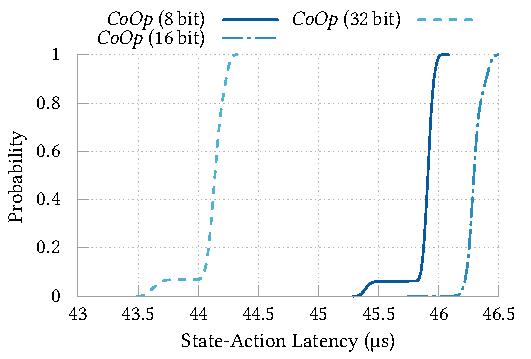
\includegraphics{../plots/build/rl-perf-tester/latency-cumul}
			\vspace{-10pt}
		}
		\caption{\approachshort's \Coopfw{} design achieves consistent, tight latency bounds.}
	\end{subfigure}
	\hspace{0.05\linewidth}
	\begin{subfigure}{0.45\linewidth}
		\resizebox{1.0\linewidth}{!}{
			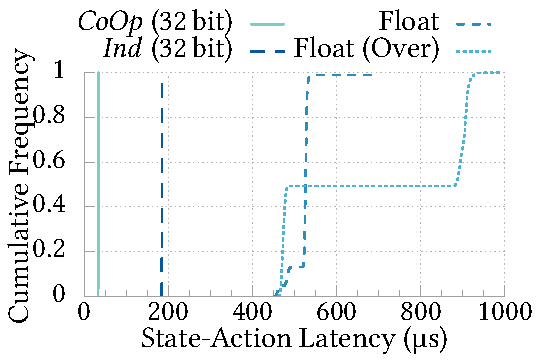
\includegraphics{../plots/build/rl-perf-tester/latency-cumul-broad}
		}
		\caption{Tail latencies suffer in hosts---particularly when oversubscribed.}
	\end{subfigure}
	\caption{Cumulative state-action latency plots for \approachshort{} and host-based execution at different quantisation settings.\label{fig:lat-cumul}}
\end{figure}

%Automatic optimisation, control, and defence of networks are at last becoming commonplace.
%Data-driven networking has led the charge in traffic optimisation, congestion control and packet classification via adaptive techniques such as \emph{reinforcement learning} (RL), where every change and its measured effects further improve future decisions.
%Considering that the network evolves in its use and deployed protocols, this flexibility is essential.
%Yet data-driven methods suffer from a key weakness: they are dependent on both the recency and accuracy of input state.
%An out-of-date view of the world will lead to suboptimal choices, as will long processing times.
%These can result in worse performance and slower adaptation to the evolving network.
%
%Programmable dataplanes and in-switch compute, then, hold promise for integrating these new techniques in a feasible and efficient manner (beyond dedicated servers or virtualised network functions). For RL, key tasks include policy evaluation, online training, state collection, and action execution -- each of these introduces some degree of sensitivity to state accuracy. Ideally then, all logic would run on these programmable devices. Yet, there is often a finite budget in microcode/FPGA space, per-packet processing times, and available cores for execution. Moreover, necessary hardware, such as floating-point units, is unavailable in almost all cases.
%
%The precise costs and trade-offs which operators and designers must make have yet to be identified. This follows from a design space explosion induced by many necessary workarounds. For instance, quantisation or fixed-point arithmetic will allow training and control on all devices, but introduces further questions: what degree of quantisation is most appropriate? What effect would this have on training accuracy, communications cost, or storage requirements? More concerns arise when we consider core allocation, local vs. distributed training, and reliable lightweight communication in multi-agent scenarios. In all cases, network operators will not consider tools which affect underlying traffic.
%
%I aim to examine the effects of these choices on an existing RL-based DDoS attack mitigation system. To protect legitimate traffic, this controls packet drop and filtering for each flow using individual metrics observed by RL agents at ingress routers, and load measurements from several points along the path taken by the flow in question. The examined metrics include the throughput and latency of its individual components alongside system metrics: flow arrival-to-judgement time, and knowledge propagation time. Beyond this, it's crucial to identify what we can implement on pure P4-capable hardware. While extensions to P4 are fairly common in commodity hardware, the need for full design access (as in NetFPGA) or Micro-C (as in Netronome SmartNICs) represent a break from the clean, loop-free semantics of P4. As the market matures, these may represent different feature classes and price points.
%
%I will discuss early development efforts (including challenges and results) on the Netronome Agilio SmartNIC, which supports the P4 language as well as some degree of arbitrary microcode. I intend to present how reinforcement learning execution and network telemetry will differ in the above metrics when compared to a vNF-based deployment (i.e., software on external commodity servers).

\section{Next Steps}
We intend to measure the effects of our data format and function approximation choices on overall accuracy and convergence times for synthetic data, comparing different bit depths against tile-coded floating-point numbers and more expressive functions such as neural networks.
Moreover, we intend to build \approachshort{} into ultra low latency control scenarios, such as short-flow prioritisation or active queue management.

\begin{acks}
	%	The authors would like to thank Rhys Simpson for his comments, and for discussions on the soundness of SIMD-like optimisations.
	%	They would additionally like to thank Stefanos Sagkriotis, Mircea Iordache-\c{S}ic\u{a}, and Haruna Adoga for their comments and feedback.
	%	We thank the anonymous reviewers of SOSR'21 and XXX'22 for their comments.
	This work was supported in part by the \grantsponsor{gs-epsrc}{Engineering and Physical Sciences Research Council}{https://epsrc.ukri.org/} [grants~\grantnum{gs-epsrc}{EP/N509668/1}, \grantnum{gs-epsrc}{EP/N033957/1}].
\end{acks}

%\bibliographystyle{ACM-Reference-Format}
%\bibliography{reference}

\printbibliography
	
\end{document}